\section{Distribution}

Like for its previous games, id decided to distribute Doom following the shareware model. A small part of the game would be given away for free and players were encouraged to be copied and redistributed as much as possible. If they liked the game they could send monet directly to id Software and receive the full version.\\
\par
\cfullimage{endoom.png}{Leaving the game displays instructions to buy the game.}
\par
Ideally, to make distribution as easy as possible, the game would have fitted on one 3\nicefrac{1}{2}-inch floppy disk. Even though 650 KiB floppy reader were fading out in favor of 1,440 KiB floppies, because of the volume of assets, DooM shareware still used two disks.\\
\cfullimage{floppies.png}{Two floppies containing Doom shareware.}
\par
In the previous photo, notice how the shareware came with a guide book which had little to do with id Software. In order to maximize distribution, id Software encouraged retails and distributor to sell the shareware or embedd it however they wanted.\\
\par

\fq{Put it in a box, sell it quote needed here.}{John Romero}

\subsection{What's in the disk?}

\def\angle{0}
\def\radius{3}
\def\cyclelist{{"orange","blue","red","green"}}
\newcount\cyclecount \cyclecount=-1
\newcount\ind \ind=-1
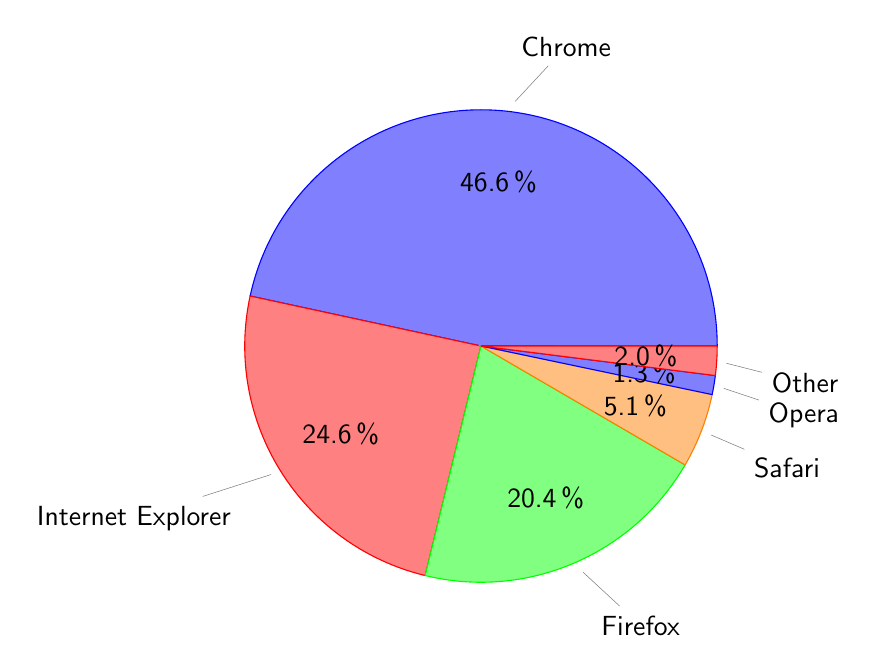
\begin{tikzpicture}[nodes = {font=\sffamily}]
  \foreach \percent/\name in {
      46.6/Chrome,
      24.6/Internet Explorer,
      20.4/Firefox,
      5.1/Safari,
      1.3/Opera,
      2.0/Other
    } {
      \ifx\percent\empty\else               % If \percent is empty, do nothing
        \global\advance\cyclecount by 1     % Advance cyclecount
        \global\advance\ind by 1            % Advance list index
        \ifnum3<\cyclecount                 % If cyclecount is larger than list
          \global\cyclecount=0              %   reset cyclecount and
          \global\ind=0                     %   reset list index
        \fi
        \pgfmathparse{\cyclelist[\the\ind]} % Get color from cycle list
        \edef\color{\pgfmathresult}         %   and store as \color
        % Draw angle and set labels
        \draw[fill={\color!50},draw={\color}] (0,0) -- (\angle:\radius)
          arc (\angle:\angle+\percent*3.6:\radius) -- cycle;
        \node at (\angle+0.5*\percent*3.6:0.7*\radius) {\percent\,\%};
        \node[pin=\angle+0.5*\percent*3.6:\name]
          at (\angle+0.5*\percent*3.6:\radius) {};
        \pgfmathparse{\angle+\percent*3.6}  % Advance angle
        \xdef\angle{\pgfmathresult}         %   and store in \angle
      \fi
    };
\end{tikzpicture}